\section{Preliminaries} \label{sec:preliminaries}
In this section, we formalize our approach to event detection.
We first describe the accompanying notations in section~\ref{sec:notations} which will be used throughout the paper.
Then we formally present our research problem statement, provide a brief comparison of our approach to a conventional solution, and review the challenging issues that are relevant to an event detection problem.
\subsection{Notations}
\label{sec:notations}
Let's assume we are given an undirected, weighted graph $\mathbf{G}(V,E,W;f)$, where $V=\{v_0,v_1,...,v_{N-1}\}$ represents the set of $N$ cities, $E$ refers to the connections between neighboring cities, and $W$ is a vector of non-negative weights associated with each edge $e_{ij}\in E$ as a function of geographical distance between a pair of vertices $(v_{i}, v_{j})$. The function, $f: V \rightarrow {\mathbb{R}}^N$ maps the vertices of graph $\mathbf{G}$, and $f(n)$ stands for the value on the vertex $v_n$. Graph $\mathbf{G}$'s adjacency matrix $\mathbf{A}$ is of size $N\times N$, where each element $a_{ij}$ is represented as:
\begin{equation}
a_{ij} = \left\{ \begin{array}{rl}
 w_{ij} &\mbox{ when $e_{ij}\in {E}$} \\
  0 &\mbox{ otherwise}
       \end{array} \right.
\end{equation}
Here, $\mathbf{A}$ is symmetric since $a_{ij}=a_{ji}$.
Let $d_i=\sum\limits_{v_j \in V}a_{ij}$ be the sum of all edge weights that are incident on $v_i$ and $\mathbf{D}$ be the diagonal matrix denoted as $\mathbf{D}=diag\{d_1,d_2,\ldots,d_N\}$. A Laplacian matrix $\mathcal{L}$ is defined as $\mathcal{L}=\mathbf{D-A}$. It is a symmetric matrix and has real eigenvalues $\lambda_{i}$ such that $0 = \lambda_{0} < \lambda_{1} \leq \lambda_{2} \leq \ldots \leq \lambda_{N-1} = \lambda_{max}$ and a complete set of $\mathcal{L}$'s normalized eigenvectors~\cite{bapat2010graphs} $\chi_{i}$ for $i=0,1,2,...,N-1$ described by:
\begin{equation}
\label{eq:eigenvalues}
\mathcal{L}\chi_{i}=\lambda_{i}\chi_{i}
\end{equation}
Obviously, $\chi_o(n)=\frac{\vec{\textbf{1}}}{\sqrt{N}}=\frac{1}{\sqrt{N}}\{1,1,...,1\}$, and is called direction component of $\mathbf{G}$.

\vspace{-1mm}
\paragraph{\textbf{Absenteeism Score}}
Although the raw volume of user interactions is a good indicator of users' online activities, it can be noisy and often exhibits a strong temporal dependence~\cite{cho2011friendship}.
For example, in Twitter, the number of user interactions tend to peak later in the day.
This can be attributed to the fact users tweet typically at home after work or school.
In order to differentiate event-related absenteeism from such noisy signals that arise from the periodicity of users' daily activities, we need to remove these artifacts from our time series data.
Empirically, tweeting locations can be modeled as a Gaussian distribution, which allows us to transform the raw counts of tweets from a given city, $v_{i}$, at time interval, $t$, into a \textit{z-score} measure, and in turn to calculate its \textit{absenteeism score} as:
\begin{equation}
	\label{eq:zscore}
	\begin{array}{l}
		f^t(i;T) =(X^t_i-\mu)/{\sigma}
	\end{array}
\end{equation}
, where $i$ denotes the index of the vertex, $X^t_i$ is the tweeting volume at time interval $t$, $\mu$ is the trailing $T$-day moving average of the volume at time $t$, and $\sigma$ is the standard deviation of that average volume.
Here, a positive absenteeism score indicates a high levels of user activity, while a negative score indicates lower levels in activity.
For the experiments described later in the paper, we set the value of $T=30$ days. The notation for absenteeism function $f^t(i;T)$ is simplified to $f$ when $t$ and $T$ are obvious from the context.
\subsection{Graph Anomaly}
\label{sec:Graph_Anomaly}
%Classic wavelet is called mathematical microscope since it is capable of showing signal abnormality with different scales.
%In the case of complex networks, graph wavelets render the graph with good localization properties both in frequency and vertex (i.e. spatial) domains. Their scaling property allows us to zoom in/out of the underlying structure of the graph.
According to Equation~\ref{eq:eigenvalues}, eigenvalues of Laplacian matrix $\mathcal{L}$ can be presented as:
\begin{equation}
\label{eq:lambda}
\lambda_{l}=\chi_{l}^T\mathcal{L}\chi_{l}= \sum_{e_{mn}\in E} w_
{mn}[\chi_{l}(m)-\chi_{l}(n)]^2
\end{equation}
$\lambda_l$ summarizes all the eigenvector deviations on any directly connected vertex $v_m$ and $v_n$ in $\mathbf{G}$. Since each term in the summation of the right-hand side is non-negative, the eigenvectors associated with smaller eigenvalues are smoother; i.e., the component differences between neighboring vertices are
small. As the eigenvalue increases, larger differences in neighboring
components of the graph Laplacian eigenvectors may be present.
Hence, for larger $\lambda_l$, its corresponding eigenvector, $\chi_l(n)$, has larger deviation among connected vertices~\cite{shuman2015vertex}. For this reason, we call $\{(\lambda_l;\chi_l)\}$ the graph anomaly pattern (also called Fourier frequency by some researchers) of $\mathbf{G}$. As mentioned above, $\chi_0(n)$ is the direct component of $\mathbf{G}$ since $\chi_0(i)=\frac{1}{\sqrt{N}}$ for any $v_i\in V$.


It is useful to analyze $f$ by taking into account the intrinsic geometric structure of the graph $\mathbf{G}$. In order to identify and exploit structure of $f\in \mathbb{R}^N$, the spectral graph $\sigma({\mathcal{L}}):=\{\chi_l\}_{l=0}^{N-1}$ can be used as a dictionary of atoms~\cite{shuman_ACHA_2013}. Thus, $f$ can be decomposed as a linear combination of $\{\chi_l\}_{l=0}^{N-1}$ as
\begin{equation}
\label{eq:graphFourier}
f(n)= \sum\limits_{l=0}^{N-1}\hat{f}(l)\chi_l(n)
\end{equation}
, where
\begin{equation}
\label{eq:graphFourier1}
\hat{f}(l):= \sum\limits_{n=0}^{N-1}\chi^*_l(n)f(n)
\end{equation}
$\hat{f}(l)$ is the inner product of $f$ and anomaly pattern $\chi_l$, and is called the graph anomaly degree in this paper, and is also called the corresponding Fourier coefficient.


\subsection{Generalized Graph Anomaly}
\label{sec:Generalized_Graph_Anomaly}
Equation~\ref{eq:graphFourier1} gives a clear representation of the anomaly patterns in $f(n)$ based on graph.  As discussed in section ~\ref{sec:Graph_Anomaly}, $\lambda_l$ only summarizes all deviations among all the direct connected vertices in graph $\mathbf{G}$.
However, in many applications,
deviations among vertices which are not connected directly might also carry important values. Taking social media network for instance, human behavior is not only being affected by his/her direct connected friends, but also by some ``far distance" friends in the network. Generalizes graph anomaly considers the deviations among all vertex pairs, which even not being connected directly, as long as they are close enough to each other.


Let $d_G(m,n)$ denote the minimum number of edges for any paths connecting $v_m$
and $v_n$ in graph $\mathbf{G}$, and $d_G(m,n)$ can be written as:
\begin{equation}
d_G(m,n)=\underset{p}\arg\min\{k_1,k_2,k_3,...,k_p\}
\end{equation}
subject\hspace{1mm}to
\begin{equation}
m=k_1, n=k_p, \hspace{1mm}and\hspace{1mm} w_{k_r,k_{r+1}}>0 \hspace{1mm} for \hspace{1mm} 1\leq r<p
\end{equation}
Note that $d_G$ disregards the values of the edge weights.
\newtheorem{thm}{Theorem}
\newtheorem{lem}[thm]{Lemma}
\begin{lem}
\label{lem:1}
Let $\mathbf{G}$ be a weighted graph, $\mathcal{L}$ the graph Laplacian and $p$ > 0 an integer. For any two
vertices $v_m$ and $v_n$ in graph $\mathbf{G}$, if $d_G(m,n) > p $ then $\mathcal{L}^p
(m,n) = 0$.
\end{lem}
The comprehensive proof of lemma~\ref{lem:1} can be found in~\cite{hammond2011wavelets}. $\mathbf{G}^p(V^p,E^p)$ denotes the graph with Laplacian matrix $\mathcal{L}^p$, and $\rho_{mn}$ denotes the weight of edge $e_{mn}$, where $e_{mn}\in E^p$. Obviously, $V^p=V$. According to the properties of  positive semi-definite, the eigenvalues and eigenvectors of $\mathcal{L}^p$ are $\{(\lambda_l^p;\chi_l)\}$, where $0\leq l \leq {N-1}$. According to Equation~\ref{eq:lambda}, for $\mathcal{L}^p$, we have
\begin{equation}
\label{eq:lambda2}
\lambda_{l}^p=\chi_{l}^T\mathcal{L}^p\chi_{l}= \sum_{e_{mn}\in E^p} \rho_
{mn}[\chi_{l}(m)-\chi_{l}(n)]^2
\end{equation}
Further, according to lemma~\ref{lem:1}, if $d_G(m,n)>p$, then $\mathcal{L}^p(m,n)=0$, which equivalently means $\rho_{mn}=0$. Hence, $\lambda_l^p$ only summarizes deviations among all vertex pairs which are closer than $p$ edges in graph $\mathbf{G}$. For this reason, we call $\{(\lambda_l^p;\chi_l)\}$ the generalized graph anomaly pattern of $\mathbf{G}$.

\subsection{Problem Statement}
\label{sec:problemformulation}
In this paper, we focus on the problem of event detection from online social networks, based on the absenteeism behavior observed in user activity in geographically proximal communities or group of cities.
Conventionally, this problem can be described as following: \emph{given a graph and \textit{absenteeism score} vector, $\mathbf{G}(V,E,W;f^t)$ at time interval $t$, select a subset $\Sigma \subseteq V$, such that
\begin{eqnarray}
 \label{eq: problem}
    \Sigma=\underset{P\subseteq V, P \mbox{ is compact}}{\arg\min}\ \ \sum_{v_k\in P} {f(k)}
\end{eqnarray} }

A general solution to this problem is using a combinatorial optimization technique, where by defining a constrained objective function over a network one can identify subset of vertices which maximize the corresponding function~\cite{rozenshtein2014event}. Therefore, Equation~\ref{eq: problem} can be modified as:
\begin{eqnarray}
 \label{eq: problem_conventional}
    \Sigma=\underset{P\subseteq V}{\arg\min}\ \ \sum_{v_k\in P} {f(k)}+\lambda \mu(P)
\end{eqnarray}
, where $\mu(P)$ is the compactness penalty function of $P$ (e.g., the sum of distances among
all pairs of the vertices in $P$~\cite{rozenshtein2014event}), and $\lambda$ is the regularization parameter.
Such methods suffer from the following issues:
\vspace{-1.5mm}
\begin{enumerate}
\item To define and measure the compactness of subset $P\subseteq V$ is challenging, considering the exponential varieties of complex graphs.
\item To determine a suitable regularization parameter $\lambda$ in the objective function is ambiguous, because simply combining multiple physically different concepts in the objective function makes the optima sensitive to $\lambda$.
\item To solve this objective function is often a \textbf{NP-hard} problem, which makes it unpractical in many real world applications. Sometimes, even the approximate solutions are of high computation complexity, if there are any.
\end{enumerate}
\vspace{-1.5mm}
In contrast, our approach proposes a novel, absenteeism based events detection algorithm in social networks using spectral graph wavelet theory.
The graph wavelets focus on the intrinsic geometric structure of the graph by transversing each vertex $v_i\in V$, and mining the topological information of both local and globally centered vertices supports the ability to conduct a multiscale analysis.
In addition, the graph wavelet approach does not introduce any ``subjective'' objective functions or other compactness concepts, and thus provides a fair and low computational method in terms of complexity for identifying abnormal group behavior in a wide variety of application scenarios.


%\begin{figure}[h]
%	\centering
%    {
%		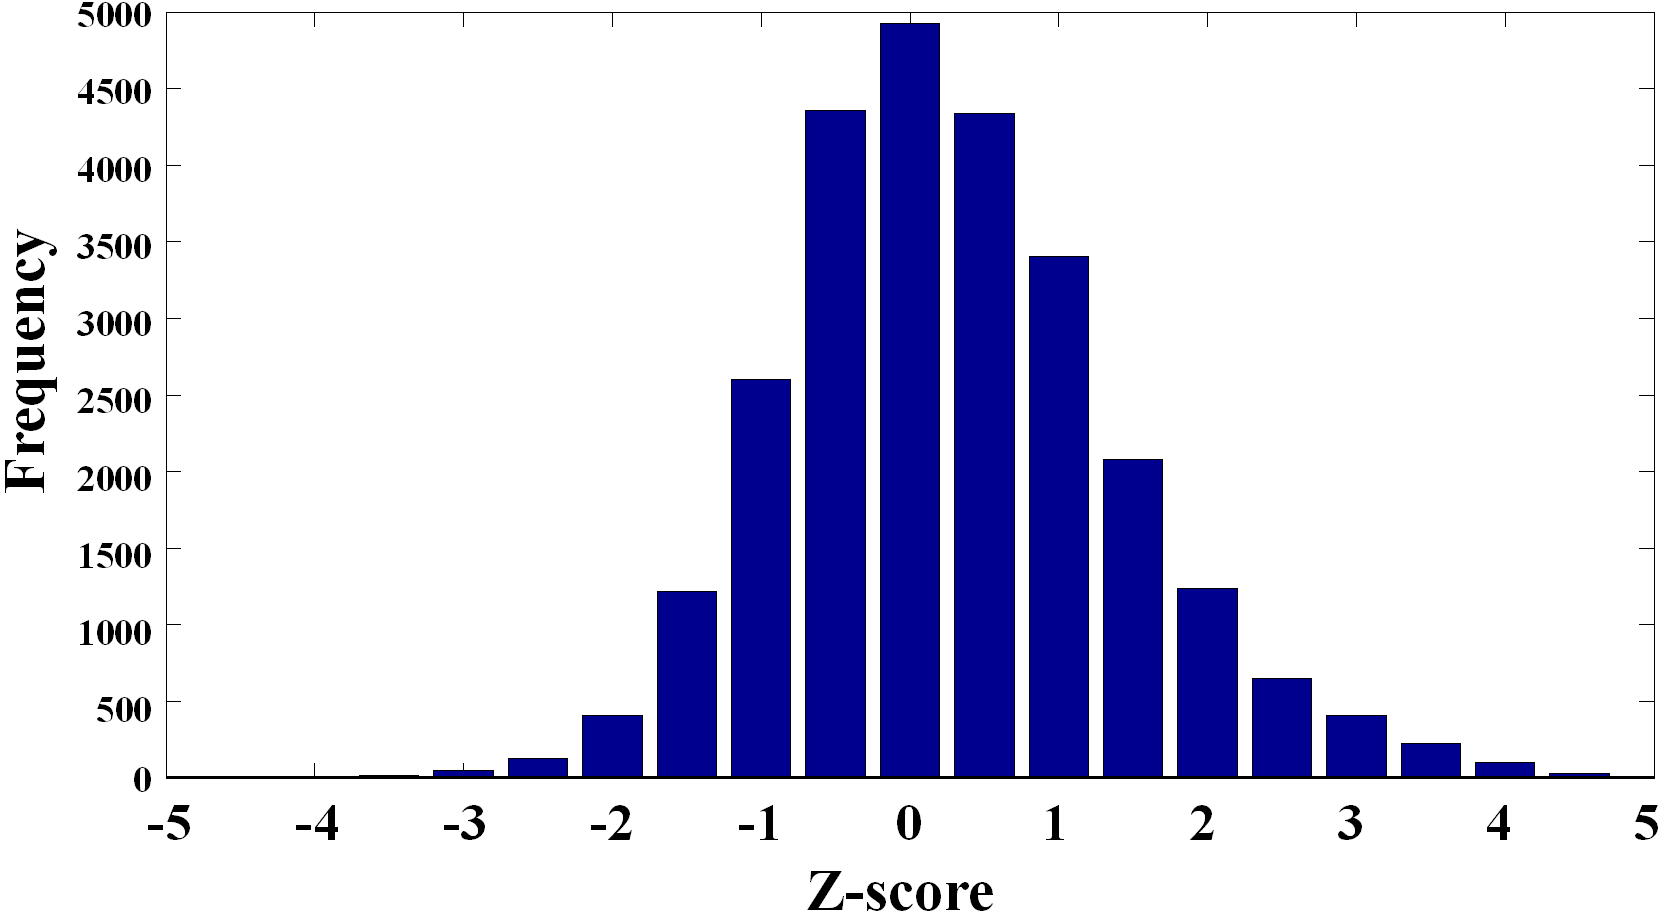
\includegraphics[width=2in] {figures/Z-Score-distribution.png}
%		\label{fig:distribution}
%	}
%	\caption{ Z-score distribution of city Sao Paulo, Brazil from Aug 1, 2012 to January 30, 2014 with time interval of five minutes. }
%	\label{fig:zscore-distribution}
%\end{figure}
